\clearpage
\section{Phase-space contraction of the damped pendulum}
\begin{colbox}
	The damped pendulum obeys
	\begin{equation}
		\ddot{\theta}=-\gamma\dot{\theta}-\frac{g}{L}\sin\theta,\qquad\gamma>0
	\end{equation}
	\begin{enumerate}
		\item Rewrite the equation as a first-order system in the phase-space coordinates. Check if the phase space area is conserved by the flow. Does the answer depend on the point you consider?
		\item Describe qualitatively, in a short paragraph, how the pendulum moves in time for different initial conditions. Sketch the corresponding phase portrait in the (\(\theta,\nu\)) plane: identify the fixed points, indicate which are stable and which are unstable, and draw a few representative trajectories. How does the addition of dissipation change the phase space portrait?
	\end{enumerate}
\end{colbox}
\subsection{First order system}
Using the definition \(\nu = \dot{\theta}\) we get the system
\begin{align}
	\dot{\theta} = \nu && \dot{\nu} = -\gamma\nu - \frac{g}{L}\sin\theta
\end{align}
To check whether the phase space area is conserved, we can take the divergence of the system
\begin{equation}
	\div{\vb{f}} = \div{\ins{\nu,-\gamma\nu-\frac{g}{L}\sin\theta}} = 0-\gamma < 0
\end{equation}
So the phase space area shrinks. This does not have any dependence on the phase space point at which we're at (with the trivial exception of (0,0)). This also makes sense, as a damped pendulum will always lose energy and tend to eventually rest.
\subsection{Qualitative Explanation}
\emph{I am assuming most of this subsection deals with an undamped pendulum. I also apologize for the drawings being made in paint, I did not have access to my iPad.}

\begin{wrapfigure}[16]{r}{0.5\textwidth}
	\begin{center}
		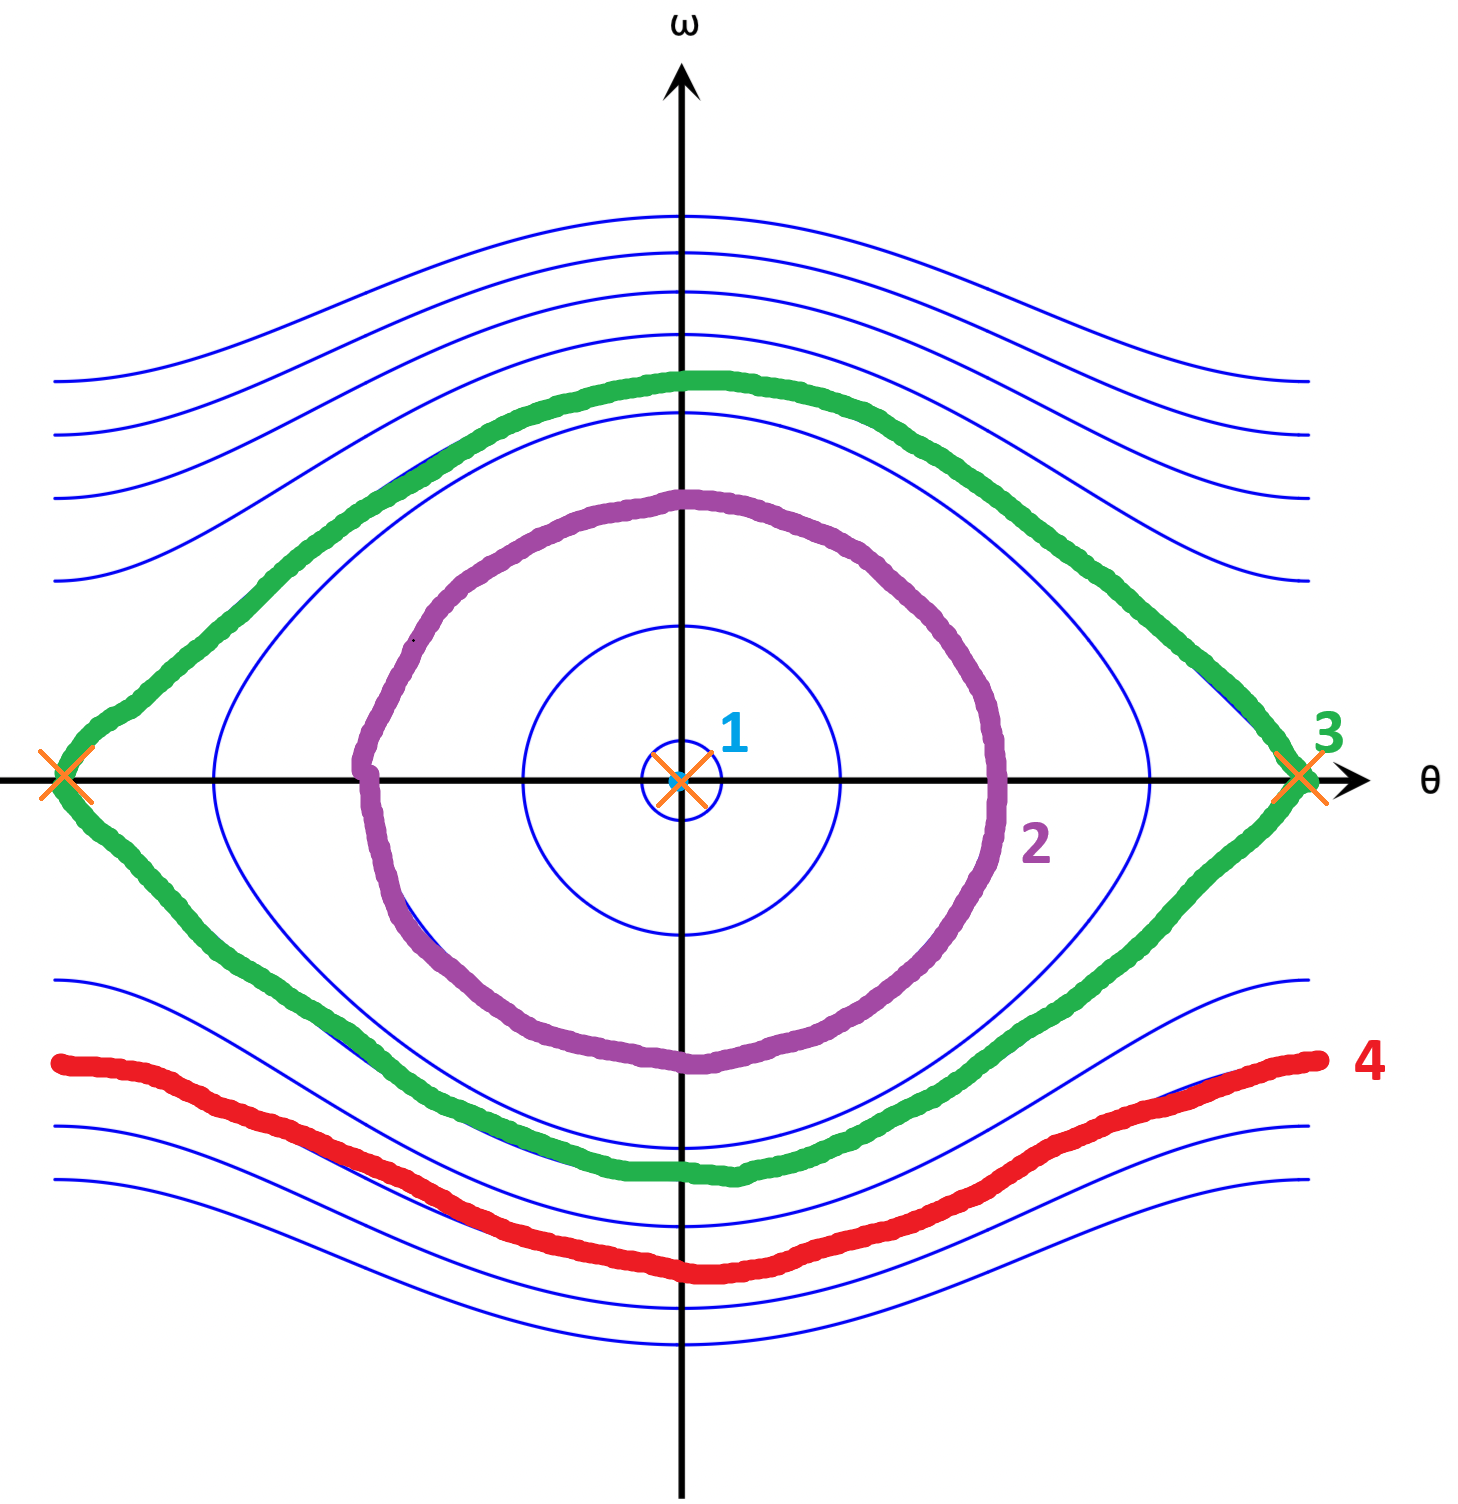
\includegraphics[width=0.5\textwidth]{phasespace.png}
	\end{center}
\end{wrapfigure}
There are 4 sets of starting conditions which can be viewed as different. The trivial is that the pendulum begins at (0,0) in phase space (marked 1 in the sketch), in which case it remains static at rest over time. The next starting conditions is in the area where the pendulum's motion can be well approximated with the small angle approximation (marked 2 in the sketch). There the pendulum behaves as we know pendulums. The third set of starting conditions is such that the phase space line for the movement is still closed by the angles reached by the pendulum are too great for the small angle approximation (marked 3 in the sketch). In this case the pendulum still rocks back and forth, but in a more complex way. The last set of starting conditions is such that the angular velocity of the pendulum is too great for gravity to overcome it and reverse direction, making the pendulum rotate in one direction (marked 4 in the sketch). The fixed points are marked with an orange X. The fixed point at (0,0) is stable, while the two others are unstable.

Adding dissipation would change the phase space portrait by curving all lines towards the center, disallowing any trajectory which does not eventually tend towards (0,0).